\documentclass[border=4pt]{standalone}
\usepackage[T1]{fontenc}
\usepackage{helvet}
\renewcommand\familydefault{\sfdefault}
\usepackage{tikz}
\usetikzlibrary{positioning,arrows.meta,shapes.misc,calc}
\usepackage{xcolor}

\begin{document}
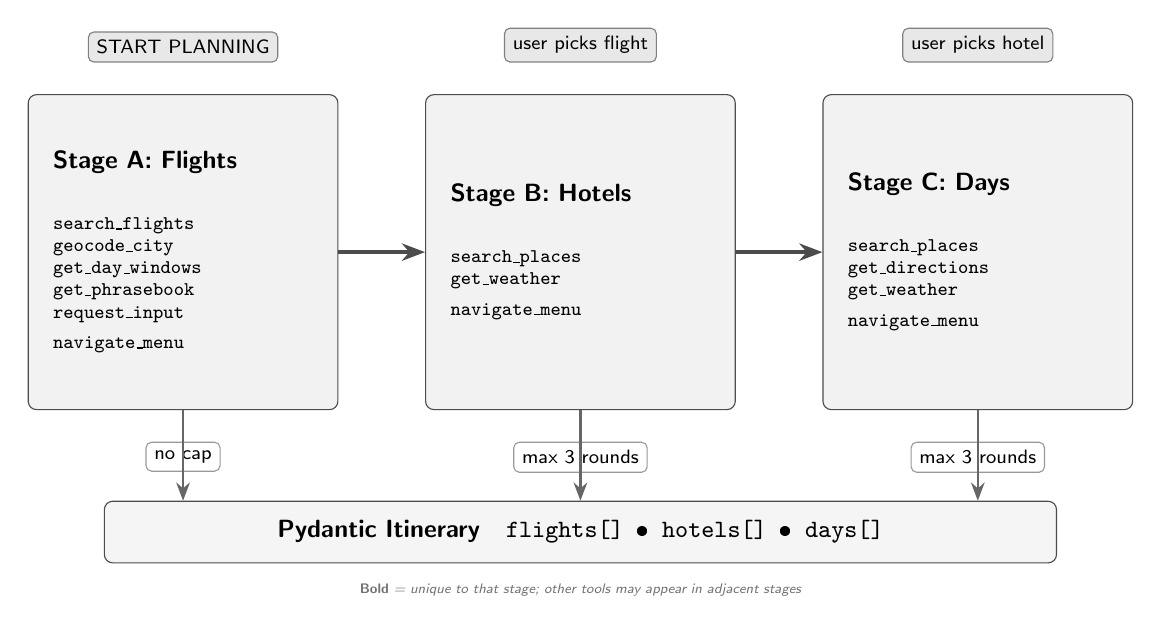
\begin{tikzpicture}[
  font=\small,
  >=Stealth,
  node distance=0.4cm,
  stagebox/.style={draw=black!70, fill=gray!10, rounded corners=3pt,
                   minimum width=3.6cm, minimum height=4.0cm,
                   inner ysep=14pt, inner xsep=9pt,
                   text width=3.3cm, align=left},
  trigbadge/.style={draw=black!50, fill=gray!18, rounded corners=2pt,
                    inner sep=3pt, font=\scriptsize, align=center},
  capbadge/.style={draw=black!40, fill=white, rounded corners=2pt,
                   inner sep=3pt, font=\scriptsize},
  itin/.style={draw=black!70, fill=gray!8, rounded corners=3pt,
               minimum width=12.0cm, inner sep=7pt, text width=11.6cm,
               align=center},
  arr/.style={->, very thick, black!70},
  droparr/.style={->, thick, black!60},
]

% ---- Stage A ----
\node[stagebox] (stageA) {%
  \textbf{Stage A: Flights}\\[14pt]
  \ttfamily\scriptsize%
  search\_flights\\%
  geocode\_city\\%
  get\_day\_windows\\%
  get\_phrasebook\\%
  request\_input\\%
  navigate\_menu%
};

% ---- Stage B ----
\node[stagebox, right=1.1cm of stageA] (stageB) {%
  \textbf{Stage B: Hotels}\\[14pt]
  \ttfamily\scriptsize%
  search\_places\\%
  get\_weather\\%
  navigate\_menu%
};

% ---- Stage C ----
% get_directions is unique to Stage C; shared tools are noted inline
\node[stagebox, right=1.1cm of stageB] (stageC) {%
  \textbf{Stage C: Days}\\[14pt]
  \ttfamily\scriptsize%
  search\_places\\%
  \textbf{get\_directions}\\%   % unique to Stage C
  get\_weather\\%
  navigate\_menu%
};

% Trigger badges above
\node[trigbadge, above=0.4cm of stageA] {START PLANNING};
\node[trigbadge, above=0.4cm of stageB] {user picks flight};
\node[trigbadge, above=0.4cm of stageC] {user picks hotel};

% Arrows between stages
\draw[arr] (stageA.east) -- (stageB.west);
\draw[arr] (stageB.east) -- (stageC.west);

% Cap badges below
\node[capbadge, below=0.4cm of stageA] {no cap};
\node[capbadge, below=0.4cm of stageB] {max 3 rounds};
\node[capbadge, below=0.4cm of stageC] {max 3 rounds};

% Pydantic Itinerary box
\node[itin, below=1.15cm of stageB] (itin) {%
  \textbf{Pydantic Itinerary}\quad
  \texttt{flights[]}\enspace\textbullet\enspace
  \texttt{hotels[]}\enspace\textbullet\enspace
  \texttt{days[]}%
};

% Drop arrows
\draw[droparr] (stageA.south) -- (itin.north -| stageA);
\draw[droparr] (stageB.south) -- (itin.north);
\draw[droparr] (stageC.south) -- (itin.north -| stageC);

% Footnote: explain bold means unique
\node[font=\tiny\itshape, anchor=north, text=black!55]
  at ([yshift=-4pt]itin.south)
  {\textbf{Bold} = unique to that stage; other tools may appear in adjacent stages};

\end{tikzpicture}
\end{document}
